\section{Predicting Behaviour}
\begin{frame}{The prediction problem}
\begin{center}
How much time will it take before a bike will be \emph{in a given hotspot}

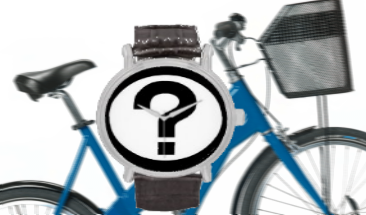
\includegraphics[width=0.8\linewidth]{graphics/biketime}
\end{center}

\end{frame}

\subsection{Modeling the system}

\begin{frame}{Simple hotspot model}
\begin{center}
\begin{figure}[H]
\begin{tikzpicture}[->,>=stealth',shorten >=1pt,auto,node distance=10cm,
  thick,main node/.style={circle,fill=blue!20,draw,font=\sffamily\Large\bfseries}]

  \node[main node] (1) {$H_1$};
  \node[main node] (2) [right of=1] {$H_2$};

  \path[every node/.style={font=\sffamily\small}]
    (1) edge [bend left] node {0.3} (2)
        edge [loop left] node {0.7} (1)
    (2) edge [bend left] node {0.6} (1)
        edge [loop right] node {0.4} (2);
\end{tikzpicture}
\caption{A Markov chain model of a system with two bike hotspots}
\label{markov:model:simple}
\end{figure}

\begin{itemize}
	\item Discrete time markov chain
	\item States represent hotspots
	\item Time- homogeneous
\end{itemize}
\end{center}
\end{frame}

\begin{frame}
\begin{center}
Where do we place the black bike?	
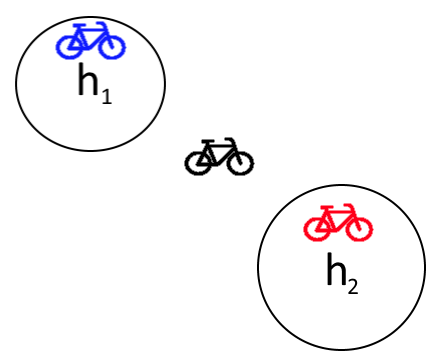
\includegraphics[scale=0.7]{graphics/world}
\end{center}
\end{frame}

\begin{frame}{Departure state model}
\begin{figure}[h]
\begin{tikzpicture}[->,>=stealth',shorten >=1pt,auto,node distance=4cm,
  thick,main node/.style={circle,fill=blue!20,draw,font=\sffamily\Large\bfseries},every node/.style={scale=0.7}]

  \node[main node] (B1) {$h_1$};
  \node[main node,font=\sffamily\small] (D1) [right = 2cm of B1] {$d_1$};
  \node[main node,font=\sffamily\small] (D2) [right of=D1] {$d_2$};
  \node[main node] (B2) [right = 2cm of D2] {$h_2$};

  \path[every node/.style={font=\sffamily\small}]
    (B1) edge [bend left] node {?} (B2)
         edge [loop left] node {?} (B1)
         edge [bend left] node[below] {?} (D1)
    (B2) edge [bend left] node {?} (B1)
         edge [loop right] node {?} (B2)
         edge [bend left] node[above] {?} (D2)
    (D1) edge [bend left] node[above] {?} (B1)
         edge [loop right] node {?} (D1)
         edge [bend left] node[below left] {?} (B2)
    (D2) edge [bend left] node[below] {?} (B2)
         edge [loop left] node {?} (D2)
         edge [bend left] node[above right] {?} (B1);
\end{tikzpicture}
\end{figure}

% VISUALIZE
% http://setosa.io/blog/2014/07/26/markov-chains/index.html
%[[0.65,0.30,0.05,0.00],
%[0.10,0.60,0.30,0.00],
%[0.15,0.00,0.50,0.35],
%[0.20,0.00,0.10,0.70]
%]
\end{frame}

\subsection{Creating the model}

\begin{frame}{}
	
\begin{center}
We want to generate the model with data from the GPS receivers on the bikes
	
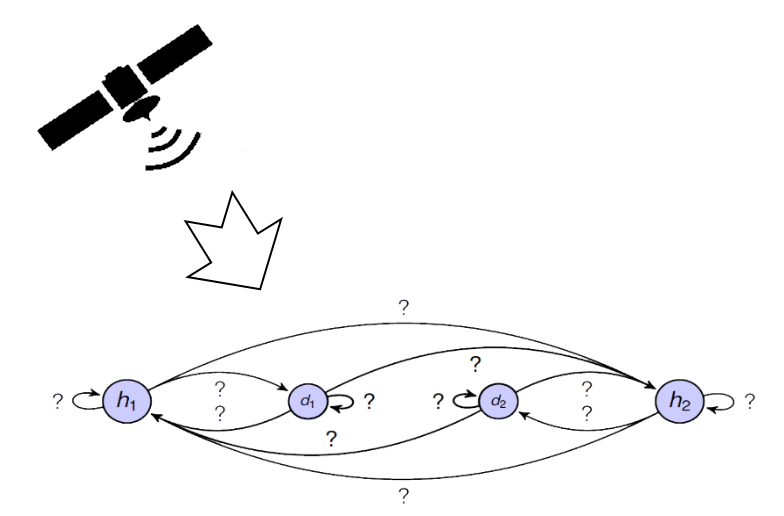
\includegraphics[width=0.8\linewidth]{graphics/build_the_model}
\end{center}

\end{frame}

\begin{frame}{Locate the bike}
	
t=0

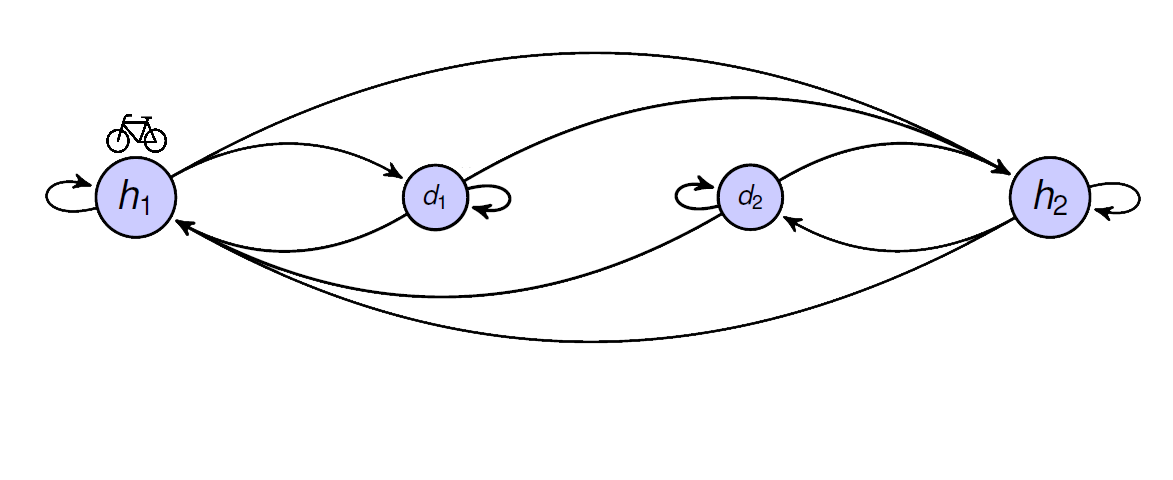
\includegraphics[width=\linewidth]{graphics/createmarkov_initial}
\[
\kbordermatrix{ 
	&  h_1 &  d_1  &  h_2  &  d_2 \\
	h_1  & 0 & 0 & 0 & 0\\
	d_1 & 0  & 0 & 0  & 0\\
	h_2  & 0 & 0   & 0 & 0\\
	d_2  & 0  & 0   & 0  & 0
}
\]
	
\end{frame}

\begin{frame}{Track the route of the bike}
t=1	
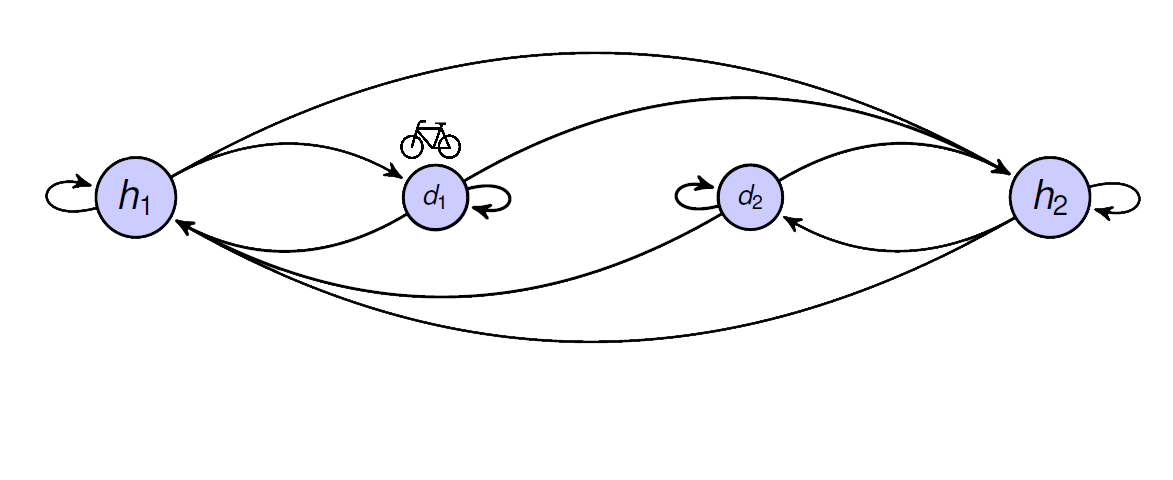
\includegraphics[width=\linewidth]{graphics/createmarkov_firststep}	
\[
	\kbordermatrix{ 
		&  h_1 &  d_1  &  h_2  &  d_2 \\
		h_1  & 0 & 1 & 0 & 0\\
		d_1 & 0  & 0 & 0  & 0\\
		h_2  & 0 & 0   & 0 & 0\\
		d_2  & 0  & 0   & 0  & 0
	}
	\]
	
\end{frame}

\begin{frame}{Track the route of the bike}
t=4
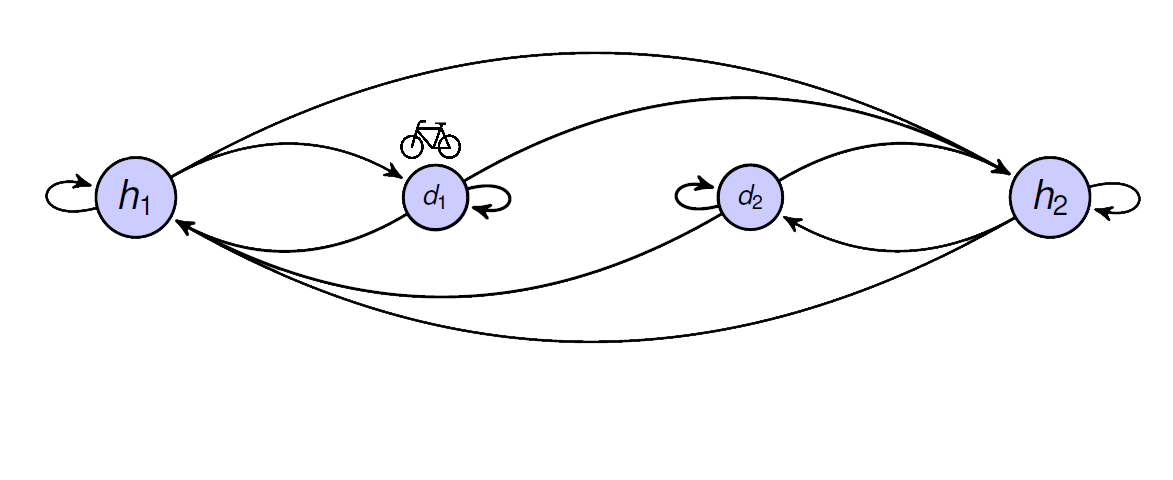
\includegraphics[width=\linewidth]{graphics/createmarkov_firststep}		
\[
	\kbordermatrix{ 
	&  h_1 &  d_1  &  h_2  &  d_2 \\
	h_1  &  0& 1 & 0 & 0\\
	d_1 & 0  & 3 & 0  & 0\\
	h_2  & 0 & 0   & 0 & 0\\
	d_2  & 0  & 0   & 0  & 0
}
\]	
\end{frame}

\begin{frame}{Track the route of the bike}
	t=5
	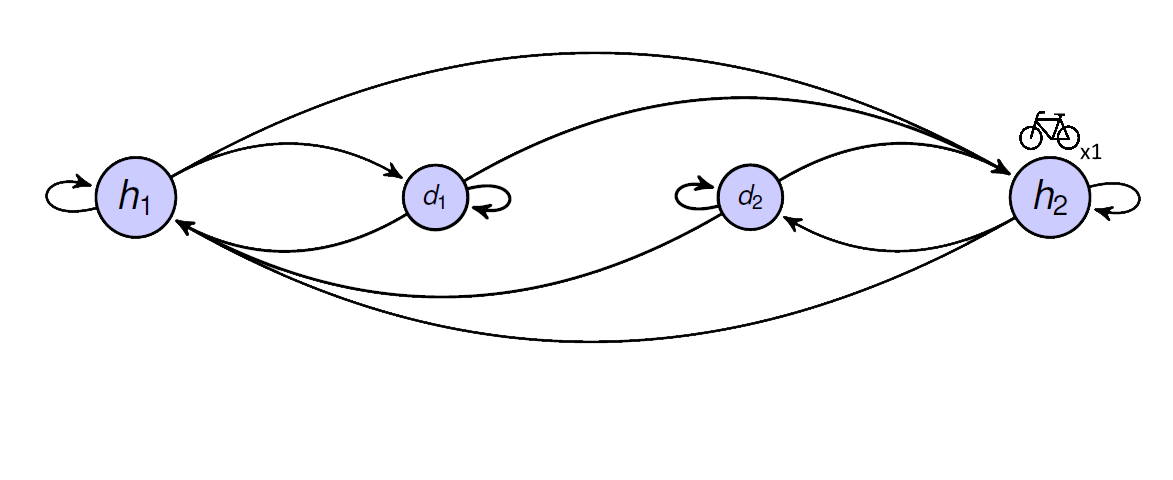
\includegraphics[width=\linewidth]{graphics/createmarkov_laststep}		
	\[
	\kbordermatrix{ 
		&  h_1 &  d_1  &  h_2  &  d_2 \\
		h_1  &  0& 1 & 0 & 0\\
		d_1 & 0  & 3 & 1  & 0\\
		h_2  & 0 & 0   & 0 & 0\\
		d_2  & 0  & 0   & 0  & 0
	}
	\]	
\end{frame}


\begin{frame}{Complete for all bikes}
t=$ t_n $
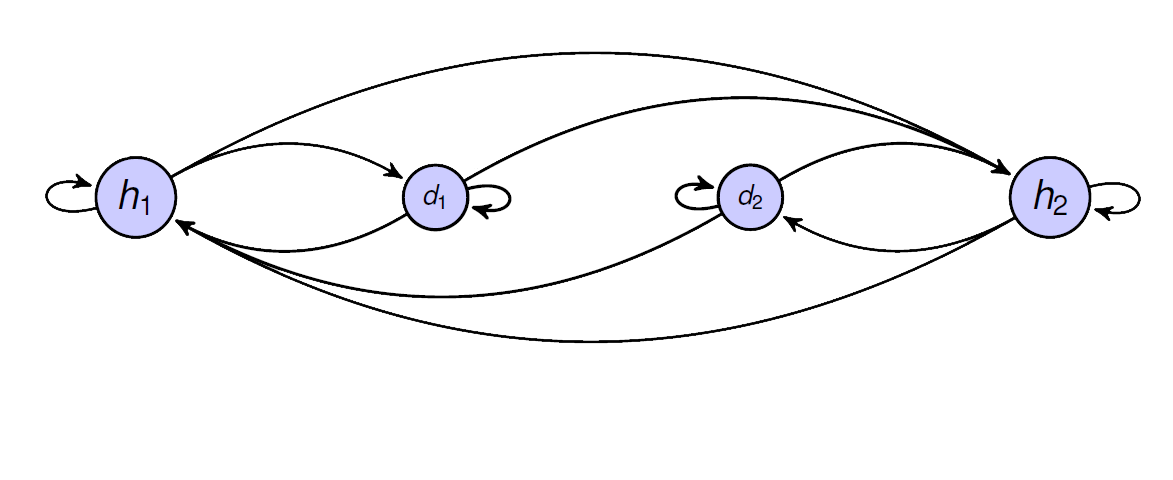
\includegraphics[width=\linewidth]{graphics/createmarkov_final}	
	\[
	\kbordermatrix{ 
		&  h_1 &  d_1  &  h_2  &  d_2 \\
		h_1  & 13 & 6 & 2 & 0\\
		d_1 & 2  & 12 & 6  & 0\\
		h_2  & 3 & 0   & 7 & 10\\
		d_2  &  4 & 0   & 2  & 14
	}
	\]		
	
\end{frame}

\begin{frame}[fragile]{Normalize the matrix}
\begin{figure}[H]
\begin{tikzpicture}[->,>=stealth',shorten >=1pt,auto,node distance=4cm,
  thick,main node/.style={circle,fill=blue!20,draw,font=\sffamily\Large\bfseries}]

  \node[main node] (B1) {$h_1$};
  \node[main node,font=\sffamily\small] (D1) [right = 2cm of B1] {$d_1$};
  \node[main node,font=\sffamily\small] (D2) [right of=D1] {$d_2$};
  \node[main node] (B2) [right = 2cm of D2] {$h_2$};

  \path[every node/.style={font=\sffamily\small}]
    (B1) edge [bend left] node {0.05} (B2)
         edge [loop left] node {0.65} (B1)
         edge [bend left] node[below] {0.3} (D1)
    (B2) edge [bend left] node {0.15} (B1)
         edge [loop right] node {0.35} (B2)
         edge [bend left] node[above] {0.5} (D2)
    (D1) edge [bend left] node[above] {0.1} (B1)
         edge [loop right] node {0.6} (D1)
         edge [bend left] node[below left] {0.3} (B2)
    (D2) edge [bend left] node[below] {0.1} (B2)
         edge [loop left] node {0.7} (D2)
         edge [bend left] node[above right] {0.2} (B1);
\end{tikzpicture}
\caption{A Markov chain model with two hotspots and departure states}
\label{markov:model:complex}
\end{figure}

% VISUALIZE
% http://setosa.io/blog/2014/07/26/markov-chains/index.html
%[[0.65,0.30,0.05,0.00],
%[0.10,0.60,0.30,0.00],
%[0.15,0.00,0.50,0.35],
%[0.20,0.00,0.10,0.70]
%]
\[
\kbordermatrix{ 
	&  h_1 &  d_1  &  h_2  &  d_2 \\
	h_1  & 0.65 & 0.3 & 0.05 & 0\\
	d_1 & 0.1  & 0.6 & 0.3  & 0\\
	h_2  & 0.15 & 0   & 0.35 & 0.5\\
	d_2  & 0.2  & 0   & 0.1  & 0.7
}
\]		

\end{frame}




\subsection{Predicting with the model}

\begin{frame}{Find the initial distribution}
\begin{center}

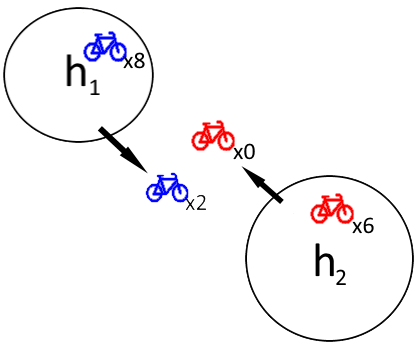
\includegraphics[scale=0.7]{graphics/initialworld2}
	
$(
\underset{h_1}{8},
\underset{d_1}{2},
\underset{h_2}{6},
\underset{d_2}{0}
)$
\end{center}
\end{frame}

\begin{frame}[fragile]
	

	
\begin{center}	
	
$ P_i \times \tau_M = P_{i+1}$\\

\begin{itemize}
	\item \textbf{$ P_i $} the initial probability
	\item \textbf{$ \tau_M $} - the markov transition function 
\end{itemize}
		
		

\[
(\underset{h_1}{8},
\underset{d_1}{2},
\underset{h_2}{6},
\underset{d_2}{0})
\times
\begin{bmatrix}
0.65 & 0.3 & 0.05 & 0\\
0.1  & 0.6 & 0.3  & 0\\
0.15 & 0   & 0.35 & 0.5\\
0.2  & 0   & 0.1  & 0.7
\end{bmatrix}
=
(
\underset{h_1}{6.3},
\underset{d_1}{3.6},
\underset{h_2}{3.1},
\underset{d_2}{3}
)
\]

\[
(
\underset{h_1}{6.3},
\underset{d_1}{3.6},
\underset{h_2}{3.1},
\underset{d_2}{3}
)
\begin{bmatrix}
0.65 & 0.3 & 0.05 & 0\\
0.1  & 0.6 & 0.3  & 0\\
0.15 & 0   & 0.35 & 0.5\\
0.2  & 0   & 0.1  & 0.7
\end{bmatrix}
=
(
\underset{h_1}{5.52},
\underset{d_1}{4.05},
\underset{h_2}{2.78},
\underset{d_2}{3.65}
)
\]


\end{center}
\end{frame}

\begin{frame}{Predicting with accumulation}
Simulating that bikes never leave the hotspot where the user is waiting

$$ \begin{bmatrix}
	{\color{red}1} & {\color{blue}0} & \color{blue} 0& {\color{blue}0}\\
	0.1  & 0.6 & 0.3  & 0\\
	0.15 & 0   & 0.35 & 0.5\\
	0.2  & 0   & 0.1  & 0.7
\end{bmatrix}
 $$
\end{frame}


\begin{frame}{Two steps of accumulation}
$$
(8, 2, 6, 0)
\begin{bmatrix}
1 & 0 & 0 & 0\\
0.1  & 0.6 & 0.3  & 0\\
0.15 & 0   & 0.35 & 0.5\\
0.2  & 0   & 0.1  & 0.7
\end{bmatrix}
=
(9.1,1.2,2.7,3)
$$
	
$$
(9.1,1.2,2.7,3)
\begin{bmatrix}
1 & 0 & 0 & 0\\
0.1  & 0.6 & 0.3  & 0\\
0.15 & 0   & 0.35 & 0.5\\
0.2  & 0   & 0.1  & 0.7
\end{bmatrix}
=
(10.225,0.72,1.605,3.45)
$$
	
\end{frame}

\begin{frame}{Comparison}
	
		Without accumulation
		$$
		(8,2,6,0)
		{\begin{bmatrix}
		0.65 & 0.3 & 0.05 & 0\\
		0.1  & 0.6 & 0.3  & 0\\
		0.15 & 0   & 0.35 & 0.5\\
		0.2  & 0   & 0.1  & 0.7
		\end{bmatrix}}^2
		=
		(5.52,4.05,2.78,3.65)
		$$
		
		With accumulation
$$
(8,2,6,0)
{\begin{bmatrix}
1 & 0 & 0 & 0\\
0.1  & 0.6 & 0.3  & 0\\
0.15 & 0   & 0.35 & 0.5\\
0.2  & 0   & 0.1  & 0.7
\end{bmatrix}}^2
=
(10.225,0.72,1.605,3.45)
$$
	
\end{frame}
